\documentclass{article}

\usepackage[utf8]{inputenc}
\usepackage{hyperref} %% for hyperlinks
\usepackage{amsmath} %% for align* environment
\usepackage{amsfonts} %% for \mathbb
\RequirePackage{graphicx} %% Include graphics
\usepackage{float} %% For float option H in figure environment

\newcommand{\Z}{\ensuremath{\mathbb{Z}}}
\newcommand{\R}{\ensuremath{\mathbb{R}}}
\newcommand{\Q}{\ensuremath{\mathbb{Q}}}
\providecommand{\C}{\ensuremath{\mathbb{C}}}
\renewcommand{\C}{\ensuremath{\mathbb{C}}}

\title{Complex Grapher Documentation}
\author{William Cooper}
\date{September 2018}

\begin{document}
	Include 'see also' section with links to domain colouring, RPN notation, shunting yard algorithm, and other things\\
	include references section
   \maketitle
	\tableofcontents
	
	\section{Introduction}
	Introduce the complex grapher package, and what it can do, with a fancy picture or two. Include a list of supported functions, scientific notation, constants e pi and i.
	
	The complex grapher application sets out to visualise complex landscapes using the domain colouring method. When learning about functions, algebra, and many other topics involving real values in mathematics, most students are introduced to a graphing package. This helps them understand the functions and how they behave. It follows that similar graphing packages for complex numbers would be useful. The complex grapher sets out to achieve this as quickly, efficiently and as simply as possible. It also ships with a few extra features that make navigating the complex landscape easier.
	
	\begin{figure}[H]
		\centering
		\makebox[\linewidth]{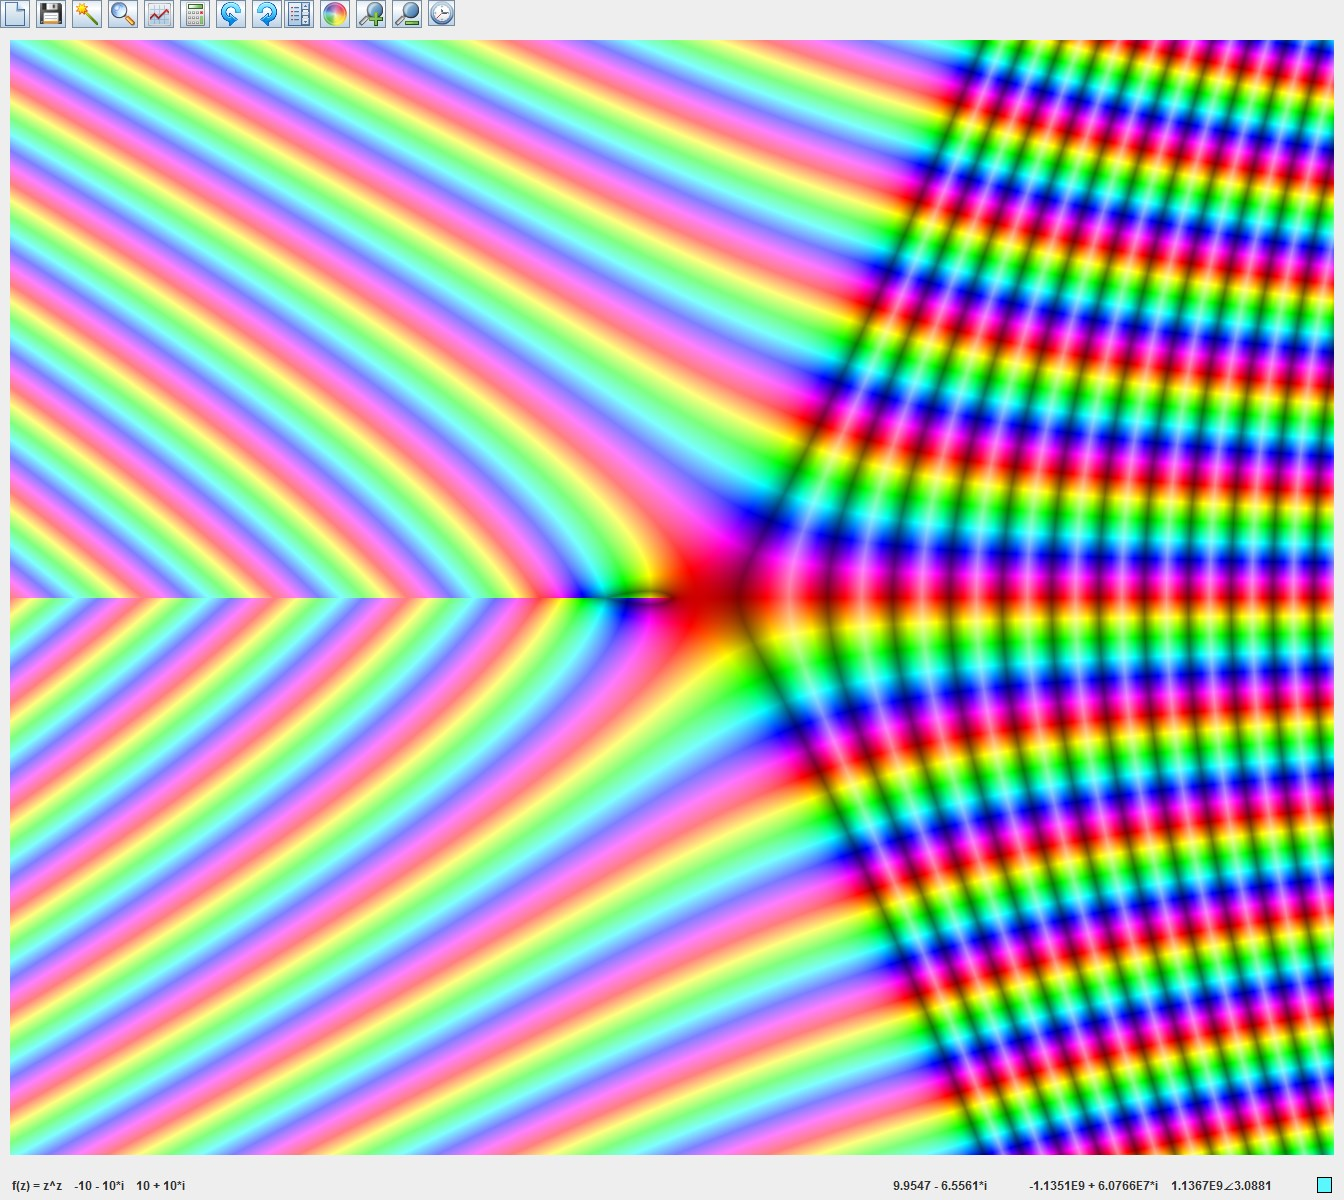
\includegraphics[scale=0.2]{z^z}}
		\textit{\caption{An image of the landscape $z^z$ with $-10-10i$ in the lower left corner, and $10+10i$ in the upper right corner.}}
		\label{graph:z^z}
	\end{figure}

	The user can input formulae composed of complex functions, along with coordinates for the bottom left corner, and the top left corner to display a landscape. The formula, and the two corner coordinates (referred to as minimum domain for the lower left, and maximum domain for the upper right henceforth) can all be expressed in terms of functions, operations and constants. For a comprehensive list of supported functions and constants, see the 'How to Use' section.

	\begin{figure}[H]
		\centering
		\makebox[\linewidth]{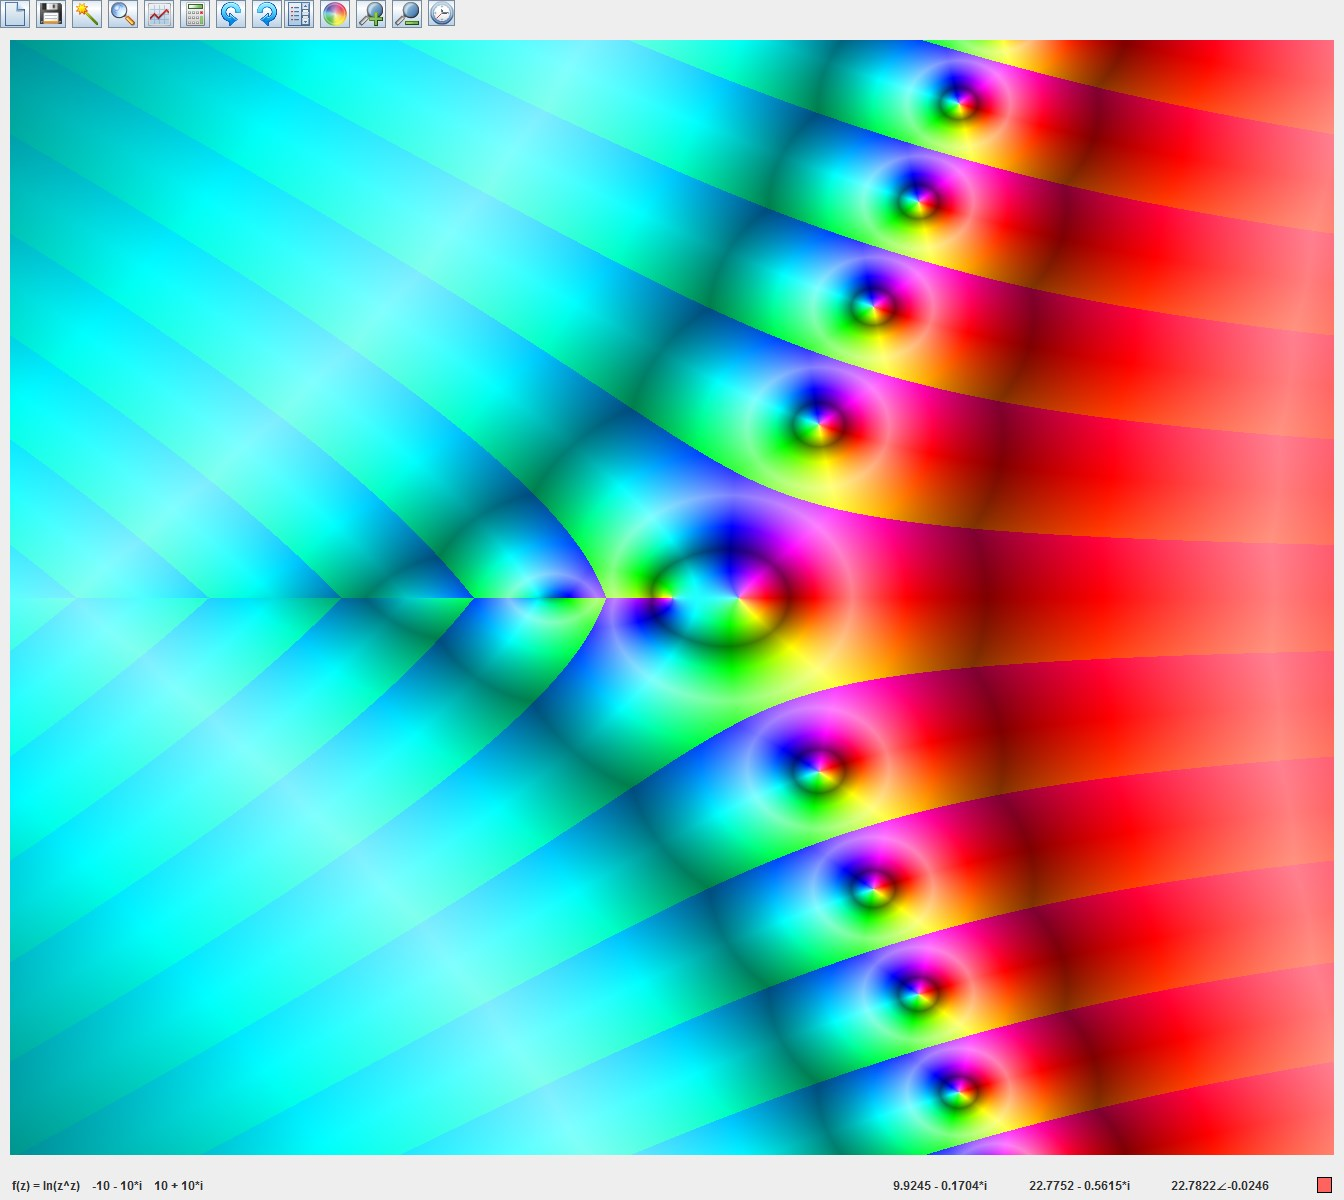
\includegraphics[scale=0.2]{ln(z^z)}}
		\textit{\caption{An image of the landscape $ln(z^z)$ with $-10-10i$ in the lower left corner, and $10+10i$ in the upper right corner.}}
		\label{graph:ln(z^z)}
	\end{figure}
	
	\section{Design features}
	\subsection{Other applications}
		This software was created out of a need to graph complex numbers to allow the user to visualise 
		complex landscape. On searching the internet for complex graphers, it quickly became apparent to the
		author that available applications were not up to a suitable standard. Some, such as the
		\href{https://www.math.ksu.edu/~bennett/jomacg/}{Math KSU} application were limited in their size and abilities. Some lacked functionality,
		(such as the \href{http://davidbau.com/conformal/#z}{David Bau} example), which has an incomplete list of trigonometric 
		functions, and no way to specify the domain). Others had so much functionality that a steep learning curve is needed to
		master these abilities,, like the \href{http://alessandrorosa.altervista.org/pages/downloads.php}{Complex Mapper}. 
		
	\subsection{Specification}
		This Complex grapher was created to solve all of these problems, by ticking the following boxes:
		
		\begin{itemize}
			\item Viewability: The user should be able to specify the size of the landscape. This means either a large form for detailed viewing, of a small form for compatibility.
			
			\item Speed: The back end should be able to create a landscape of the specified size as quickly as the host hardware can handle. Ideally this should be fast enough so the user does not notice a large delay between actions and results. Navigation events such as Pan and zoom should also be fast enough to create accurate landscapes without forcing the user to wait
			
			\item Efficiency: The code should create the landscape with minimal effort supplied from the host machine.
			
			\item Accuracy: All landscapes produced within reasonable bounds, should display information with as much accuracy as the host
			is able to supply
			
			\item Intuitive: The application should present itself with a minimal, but complete set of features. These include features for easy navigation of the landscape, as well as mathematical information on the landscape. Only core functionality should be included, that is, features the user is likely to understand and use. The use of complicated and obscure features reduced user experience. The user is advised to use generic Mathematics software to achieve these tasks.
			
			\item Compatibility: The application should be produced to run on as many operating systems as is feasible. It should also be designed to take advantage of the most powerful (or accurate) hardware available.
		\end{itemize}
	
	\section{Explanation}
	The application parses the formula into a list of tokens, and the minimum and maximum domain into complex constants that the kernel and Java code can use. The complex grapher application then uses OpenCL (using the Java wrapper JavaCL) to generate the image. First each thread is given its own unique value of $z$, the input value. The is calculated using the minimum and maximum domain, along with the width and height of the complex widget. The kernel then uses a virtual stack for each thread, when each thread activates it evaluates the expression using the postfix evaluation algorithm. Adjacent threads will access adjacent locations in memory during the stack calculations, which allows for coalesced memory access. 
	
	OpenCL is used because it allows for high level parallelism supported by many devices and vendors. It automatically selects the most appropriate device based on a prioritised criteria. The user can prioritise speed (selects the device based on the most the number of compute units) or it can prioritise accuracy (selects fastest device supporting double precision). 
	
	It is worth noting here that choosing double precision does not only allow for the most accurate results, it also allows larger and smaller values to be represented. Functions that increase quickly (such as $z^z$ mentioned earlier) will overflow and underflow faster using single precision. It is highly recommended that the user prioritise accuracy unless the computation is very slow. If the fastest device supports double precision calculations, switching priorities will have no effect on the device. When the application is executed via command line, the application will output the priority type, and which device is used.
	
	\subsection{Domain colouring}
		When graphing single variable real functions of the form, \begin{align*}
			f : &\R \to \R\\
			 &x \mapsto x,
		\end{align*} the domain and codomain are both $\R$, so any point in the space can be expressed as a coordinate in $\R^2$. These two dimensional graphs can 
		easily be represented on computers. However, taking the complex numbers as the domain and codomain means we now have to display the complex landscape
		in 4 dimensions. We solve this problem by displaying the landscape as a two dimensional image, with the real values as the x axis, and the imaginary values in 
		the y axis. Each point then represents a complex number, $f(z)$ at $(x,y)$. This complex value is displayed as a colour, with two parts - hue and lightness. Hue 
		represents the argument, and lightness the modulus. To understand how the hue is represented, recall that a complex number can be shown in an argand diagram:
		
		[insert diagram(s) of complex numbers on an argand diagram]
		
		Now imagine the colour wheel superimposed over this image. The colour in the direction of the complex number represents its hue:
		
		[insert diagram of complex numbers with superimposed colour wheel]
		
		Next we look at the lightness. To represent increasing modulus, we create rings, like those on a map. On a map, lines represent increments in height (say 10 meters).
		Lines grouped closer together represent a steeper climb in elevation (or modulus in this case) than lines grouped far apart. The main difference here is that in maps
		the increase from one line to the next is linear, whereas increases in the complex grapher landscape are geometric.
	
	\subsection{How to Use}
		Explain to the reader  how to use the basic features of the software with screenshots, followed by the more complex features.
		
	\section{How it works}
	Give a brief explanation of how it works, followed by a detailed explanation broken up into subsections. Include detailed explanation
	of coalesced memory.
   
\end{document}